% \subsection{UC37: Gestione credenziali}
% \label{sec:UC37}
% \begin{figure}[!ht]
%     \caption{Diagramma di UC37: Gestione credenziali}
%     \vspace{10px}
%     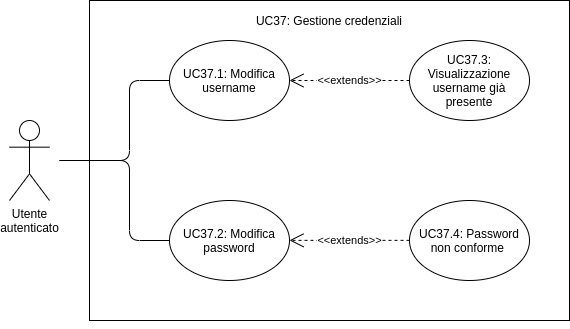
\includegraphics[scale=0.5]{../../../Images/AnalisiRequisiti/UC37}
%     \centering
% \end{figure}

% \begin{itemize}
%     \item \textbf{Descrizione:} l'utente vuole gestire le proprie credenziali;
%     \item \textbf{Attore Primario:} utente autenticato;
%     \item \textbf{Attore Secondario:} servizio di autenticazione esterno;
%     \item \textbf{Precondizione:} l'utente si trova all'interno del proprio profilo;
%     \item \textbf{Postcondizione:} l'utente può modificare le proprie credenziali;
%     \item \textbf{Scenario Principale:}
%           \begin{itemize}
%               \item  l'utente decide cosa modificare tra:
%                     \begin{itemize}
%                         \item username \underline{\hyperref[sec:UC37.1]{UC37.1}};
%                         \item password  \underline{\hyperref[sec:UC37.2]{UC37.2}}.
%                     \end{itemize}
%           \end{itemize}
% \end{itemize}

% \subsubsection{UC37.1 Modifica dell'username}
% \label{sec:UC37.1}
% \begin{itemize}
%     \item \textbf{Descrizione:} l'utente vuole modificare il proprio username;
%     \item \textbf{Attore Primario:} utente autenticato;
%     \item \textbf{Attore Secondario:} servizio di autenticazione esterno;
%     \item \textbf{Precondizione:} l'utente si trova all'interno del proprio profilo;
%     \item \textbf{Postcondizione:} l'utente può modificare il proprio username;
%     \item \textbf{Estensione:} username già presente nel database:
%           \begin{itemize}
%               \item l'utente può inserire nuovamente lo username \underline{\hyperref[sec:UC38]{UC38}}.
%           \end{itemize}
% \end{itemize}

% \subsubsection{UC37.2 Modifica della password}
% \label{sec:UC37.2}
% \begin{itemize}
%     \item \textbf{Descrizione:} l'utente vuole modificare la propria password;
%     \item \textbf{Attore Primario:} utente autenticato;
%     \item \textbf{Attore Secondario:} servizio di autenticazione esterno;
%     \item \textbf{Precondizione:} l'utente si trova all'interno del proprio profilo;
%     \item \textbf{Postcondizione:} l'utente può modificare la propria password.
%     \item \textbf{Estensione:} la password inserita non è conforme ai requisiti:
%           \begin{itemize}
%               \item L'utente può reinserire la password rispettando i requisiti \underline{\hyperref[sec:UC39]{UC39}}.
%           \end{itemize}
% \end{itemize}

\subsection{UC37: Modifica della password}
\label{sec:UC37}
\begin{itemize}
    \item \textbf{Descrizione:} l'utente vuole modificare la propria password;
    \item \textbf{Attore Primario:} utente autenticato;
    \item \textbf{Attore Secondario:} servizio di autenticazione esterno;
    \item \textbf{Precondizione:} l'utente si trova all'interno del proprio profilo;
    \item \textbf{Postcondizione:} l'utente può modificare la propria password.
    \item \textbf{Estensione:} la password inserita non è conforme ai requisiti:
          \begin{itemize}
              \item L'utente può reinserire la password rispettando i requisiti \underline{\hyperref[sec:UC39]{UC39}}.
          \end{itemize}
\end{itemize}